% ------
% METHOD
% ------

% Defining TOC's sections before content

\section{Méthodes numériques}

\subsection{CDMFT \&\;PyQCM}

\subsection{Algorithme de sous-bains}

\begin{frame}
    \vfill
    \begin{center}
        \large
        Méthodes numériques
    \end{center}
    \vfill
\end{frame}

\begin{frame}
  \frametitle{Méthodes numériques - CDMFT \&\;PyQCM}
    On choisit un amas pour lequel on calcule la fonction de Green en tenant
    compte des interactions avec le bain via $\vb{H}_{\text{AIM}}$
    \begin{align}
        \vb{G}_c^{-1}(z) = z - \vb{t}_c - \vb{\Sigma}_c(z) - \vb{\Gamma}(z).
    \end{align}
    \begin{figure}
         \centering
         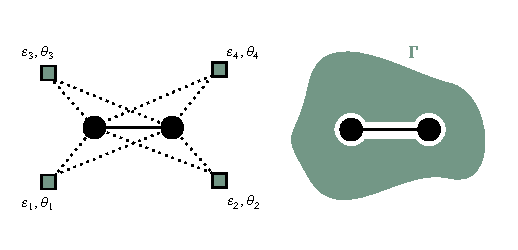
\includegraphics[scale=0.8]{./figures/theory/1D_2s_4b_bulk.pdf}
         % \caption{Amas 1D plongé dans un bain sans interactions.}
         \label{fig: amas_CDMFT}
    \end{figure}
\end{frame}

\begin{frame}
  \frametitle{Méthodes numériques - CDMFT \&\;PyQCM}
  L'effet du bain sur la fonction de Green est encapsulé dans ladite
  \textcolor{hard_green}{fonction d'hybridation $\vb{\Gamma}(z)$}
  \vspace{1cm}
  \begin{align}
    \vb{\Gamma}(z) = \Gamma_{ij,\sigma}(z) = \sum_\nu\frac{\theta_{i\nu,\sigma}\theta^*_{j\nu,\sigma}}{z - \epsilon_{\nu,\sigma}},
    \label{eq: hybridization}
  \end{align}
  \vspace{1cm}

  à l'intérieur de laquelle sont stockés les paramètres variationnels de l'algorithme CDMFT.
\end{frame}

\begin{frame}
  \frametitle{Méthodes numériques - CDMFT \&\;PyQCM}
    L'essence de la CDMFT est d'obtenir une correspondance entre
    $\vb{G}_c(z)$ et $\vb{\Bar{G}}(z)$ via \textcolor{hard_green}{l'approximation locale de la \textit{self-énergie}:}
    \begin{align}
        \textcolor{hard_green}
        {\vb{\Sigma}(\vb{\tilde{k}}, z)\longrightarrow\vb{\Sigma}_c(z),}
    \end{align}
    dans une boucle d'auto-cohérence.
    \vfill
    \pause
    Grâce au formalisme de base mixte, on calcule la fonction de Green
    \textbf{projetée sur l'amas}
    \begin{align}
        \vb{\Bar{G}}(z) = \Bigg[\frac{N_c}{N}\sum_{\vb{\Tilde{k}}}e^{i\vb{\Tilde{k}}\cdot\vb{\Tilde{r}}}\vb{G}(\vb{\Tilde{k}}, z)\Bigg]_{\vb{\Tilde{r}}=0}
        = \frac{N_c}{N}\sum_{\vb{\tilde{k}}}\frac{1}{z - \vb{t}(\vb{\tilde{k}}) - \textcolor{hard_green}{\vb{\Sigma}_c(z)}}.
    \end{align}
\end{frame}

\begin{frame}
  \frametitle{Méthodes numériques - CDMFT \&\;PyQCM}
    La fonction de distance est donnée par
    \begin{align}
      d &= \sum_{i\omega_n, \mu, \nu}W_n|(\vb{G}_c^{-1}(i\omega_n) - \vb{\Bar{G}}^{-1}(i\omega_n))_{\mu\nu}|^2 \\
        &=\sum_{i\omega_n, \mu, \nu}W_n|(\vb{\Gamma}(i\omega_n) - \vb{\Bar{\Gamma}}(i\omega_n))_{\mu\nu}|^2,
        \label{eq: dist}
    \end{align}
    où $i\omega_n$ sont les fréquences de Matsubara et $W_n$ des poids arbitraires.
    C'est grâce à cette fonction que l'on calcule la correspondance entre $\vb{G}_c(z)$ et $\vb{\Bar{G}}(z)$.
\end{frame}

\begin{frame}
    \frametitle{Méthodes numériques - CDMFT \&\;PyQCM}
    \begin{columns}
        \column{0.4\linewidth}
        \hspace{1cm}
        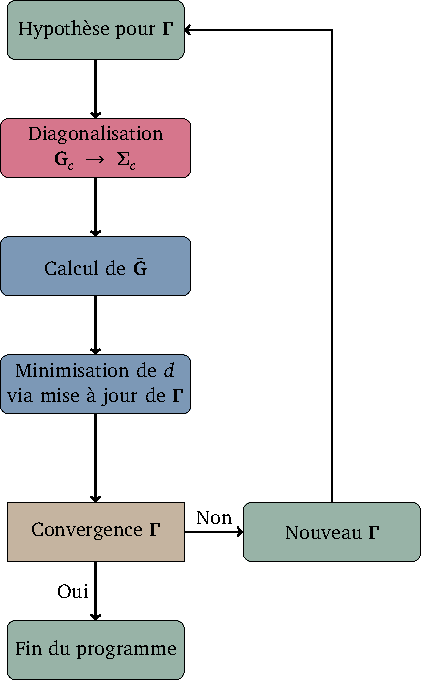
\includegraphics[scale=0.5]{./figures/theory/flow_chart.pdf}
        \column{0.6\linewidth}
        \begin{itemize}
            \item[$\diamond$] Des paramètres $\varepsilon_i, \theta_i$ arbitraires
                sont définit pour l'hybridation d'essai $\vb{\Gamma}(z)$
            \pause
            \item[$\diamond$] Solutionneur d'impureté (ED) pour accéder à
                $\vb{G}_c\to\vb{\Sigma}_c$
            \pause
            \item[$\diamond$] Calcul de la fonction de Green \textbf{projetée sur l'amas} $\vb{\bar{G}}$
            \pause
            \item[$\diamond$] Minimise la fonction de distance $d$ grâce aux paramètres de $\vb{\Gamma}(z)$
            \pause
            \item[$\diamond$] L'hybridation mise à jour est comparée à celle
                de l'itération précédente
        \end{itemize}
    \end{columns}
\end{frame}

\begin{frame}
    \frametitle{Méthodes numériques - Algorithme de sous-bains}
    L'idée est de morceler le bain en sous-bains dont un seul est impliqué dans
    la diagonalisation à chaque itération
    \begin{align}
      \vb{G}^{-1}_{c_i}(z) = z - \vb{t}_{c_i}(z) - \vb{\Gamma}_{c_i}(z) - \vb{\Sigma}_{c_i}(z)
    \end{align}
    \begin{figure}
         \centering
         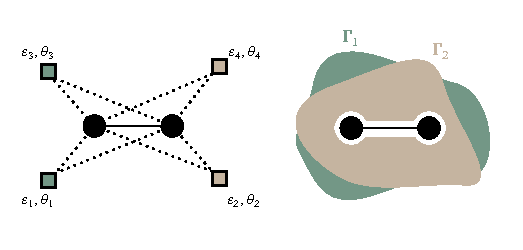
\includegraphics[scale=0.75]{./figures/theory/1D_2s_4vb_bulks.pdf}
         % \caption{Amas 1D plongé dans deux sous-bains sans interactions.}
         \label{fig: amas_CDMFT_virtual}
    \end{figure}
\end{frame}

\begin{frame}
    \frametitle{Méthodes numériques - Algorithme de sous-bains}
    Cependant, que se passe-t-il avec l'approximation locale de la self-énergie?
    Plusieurs self-énergies sont valides...
    \begin{align}
      {\vb{\Sigma}(\vb{\tilde{k}}, z)\longrightarrow\cancel{\vb{\Sigma}_c(z)},}
    \end{align}
\end{frame}

\begin{frame}
    \frametitle{Méthodes numériques - Algorithme de sous-bains}
    Cependant, que se passe-t-il avec l'approximation locale de la self-énergie?
    Plusieurs self-énergies sont valides...
    \begin{align}
      \vb{\Sigma}(\vb{\tilde{k}}, z)\longrightarrow\textcolor{hard_green}{\lambda_1\vb{\Sigma}_{c_1}(z) +
      \lambda_2\vb{\Sigma}_{c_2}(z)},
    \end{align}
    \pause
    Ce qui modifie le calcul de la fonction de Green projetée et la fonction de distance
    \begin{align}
        \vb{\Bar{G}}(z) = \frac{N_c}{N}\sum_{\vb{\tilde{k}}}\frac{1}{z - \vb{t}(\vb{\tilde{k}}) - (\textcolor{hard_green}{\lambda_1\vb{\Sigma}_{c_1}(z) +
        \lambda_2\vb{\Sigma}_{c_2}(z)})}.
    \end{align}
    \begin{align}
      d = \sum_{i\omega_n, \mu,\nu}W_n|(\textcolor{hard_green}{\lambda_1\vb{\Gamma}_{c_1}(i\omega_n) + \lambda_2\vb{\Gamma}_{c_2}(i\omega_n)} - \vb{\Bar{\Gamma}}(i\omega_n))_{\mu\nu}|^2
    \end{align}
\end{frame}

\begin{frame}
    \frametitle{Méthodes numériques - Algorithme de sous-bains}
    \begin{columns}
        \column{0.25\linewidth}
        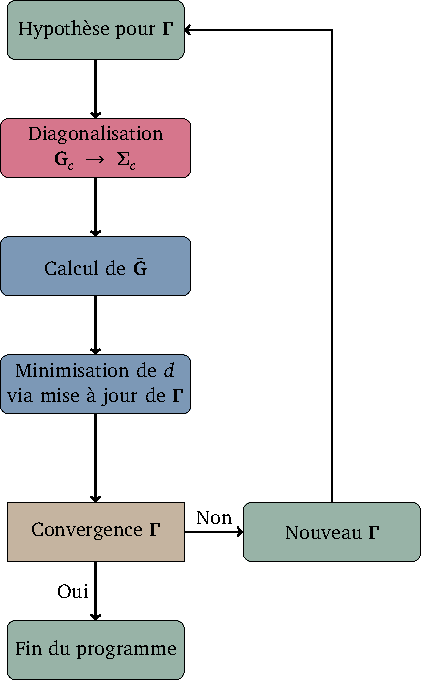
\includegraphics[scale=0.45]{./figures/theory/flow_chart.pdf}
        \column{0.05\linewidth}
        \Large
        $\longrightarrow$
        \column{0.5\linewidth}
        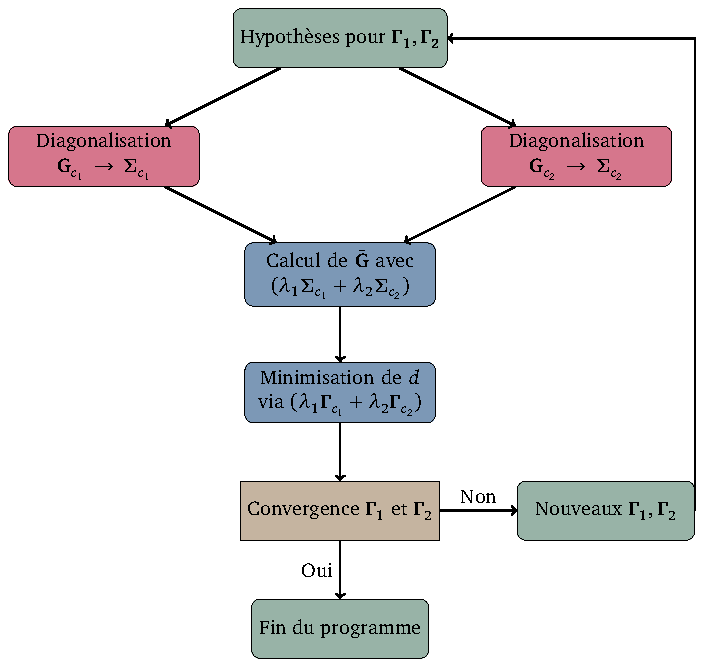
\includegraphics[scale=0.45]{./figures/theory/flow_chart_sub_baths.pdf}
    \end{columns}
\end{frame}
